% allocate 2 page
\chapter{Introduction}
\section{Motivation}
\label{section:motivation}
Pre-trained language models (PLMs) are deep neural networks trained on vast corpora, such as Wikipedia, to predict a masked-out word or sentence given the context. These models have shown effectiveness in many natural language processing (NLP) applications \cite{Devlin18BERT}. The idea of \textit{pre-train then fine-tune} approach applies the knowledge of the PLM to new downstream end-user tasks. During training, an additional neural network layer is added on top of the PLM and parameters are fine-tuned using training samples of the downstream task. However, producing high-performing models with this \emph{pre-train then fine-tune} approach with limited training data is challenging. Prompt-based learning (PL) \cite{Liu21} is a new paradigm that achieved state-of-the-art performance on a range of NLP tasks, particularly under few-shot learning scenarios where only a few training samples are available.

\begin{figure}[!ht]
    \centering
    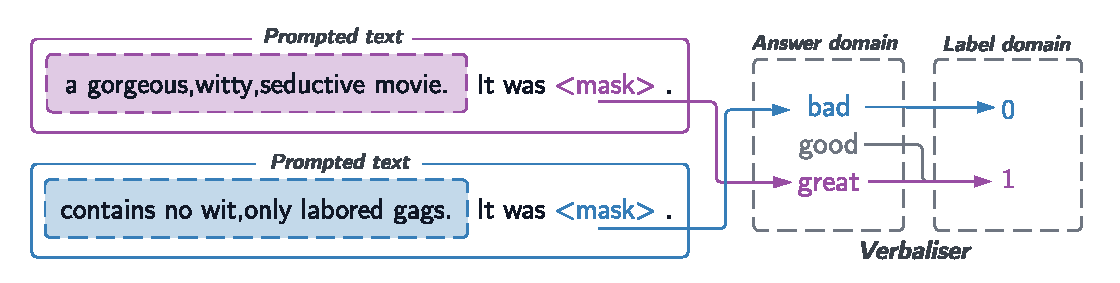
\includegraphics[width=\hsize]{figures/introduction_media/intro-pl.pdf}
    \caption{Prompt-based learning for sentiment analysis on movie reviews.}
    \label{fig:intro-pl}
\end{figure}

\vspace{-1.2em}
\paragraph{PL directly probes knowledge from PLMs} Instead of the \textit{pre-train then fine-tune} approach, PL modifies the input text, such as a movie review shown in \Cref{fig:intro-pl}, with a prompt. The prompt is a template with one or more placeholders called $<$\textit{mask}$>$ tokens. By asking the PLM to fill in the blanks, PL converts the problem into a cloze completion task. Additionally, PL incorporates a verbaliser that links candidate words (e.g., the word \textit{great}) to output labels (e.g., label \textit{1}). The verbaliser maps the optimal word the PLM selects to a label that serves as the final prediction. Without fine-tuning an extensive set of parameters, PL can more efficiently and explicitly use the knowledge in the PLM to fit the downstream task.

\vspace{-0.8em}
\paragraph{PL models are vulnerable} Advances in PL have brought the security vulnerabilities of the paradigm to the forefront. Recent research has investigated the possibilities of injecting backdoors into PLMs \cite{Lei22, Du22}. A backdoor-triggered attack can totally control or severely impact the performance of prompt-based models. By embedding backdoors into the PLM, it preserves normal model behaviour and only acts maliciously when the model encounters some pre-defined triggers in the input text. 

\vspace{1em}
This project aims to re-implement various prompt-based models, exploit their vulnerabilities under backdoor attacks and seeks to answer the following two questions:
\begin{itemize}[topsep=0pt, itemsep=0.8pt, partopsep=0pt]
    \item Under a few-shot scenario, whether one prompting model outperforms another, and why?
    \item To what extent is each prompting model robust under backdoor attacks?
\end{itemize}

\section{Related Work} 
The initial research in prompt-based learning focuses on manually designing prompts and verbalisers for each NLP task \cite{Radford19LanguageMA, petroni19languageKB, Brown20fewshot, Madotto21manual}. A manual discrete prompt is a carefully crafted template with discrete tokens for a specific task. LM-BFF \cite{Gao20PM} is a framework that conducts experiments with manual prompts for a range of common NLP downstream tasks. \Cref{fig:intro-pl} shows one of the manual discrete prompts in LM-BFF for the sentiment analysis task on movie reviews. 

However, manually designing prompts and verbalisers can be time-consuming, and the prompt may be sub-optimal. To address this, numerous methods for automatically constructing prompts are proposed: mining-based methods require access to a large text corpus to find middle words or dependency paths \cite{jiang20Auto}; prompt paraphrasing methods build on top of a manual discrete prompt, then select an optimal one from a set of paraphrased candidate prompts \cite{Yuan21Auto};  prompt generation methods convert the problem into a text generation task and applies another PLM such T5 to fill missing spans \cite{Ben-David21Auto}. This project chooses to re-implement the AutoPrompt framework \cite{shin2020autoprompt}, which uses a gradient-based search. Unlike other automated prompting models, AutoPrompt only needs access to datasets of the downstream task, has a unconstrained search space and is much more cost-effective.

Instead of using discrete tokens in the prompts, recent research treats tokens as trainable parameters in a continuous space and introduces so-called differential prompting models, or soft prompts \cite{Liu21, Lester21hz, Vu21SPoT}. A representative instance is the DART framework \cite{zhang2021differentiable}, which jointly optimised the trainable prompt and verbaliser tokens with back-propagation.

A backdoor attack is a severe security threat for deep learning models \cite{Gu17BadNets}. Since prompt-based learning inherits the vulnerabilities from the pre-trained language models (PLM), it creates opportunities to insert backdoors into the PLMs \cite{Lei22}. By poisoning the training samples with backdoor triggers, the backdoored model can establish a mapping between the trigger tokens and the target labels, preserving a high model classification accuracy but conducting misbehaviours once the trigger is added to the input text \cite{Li21backdoorsoft}.

In a backdoor attack, triggers selected are usually nonsense words (e.g., \textit{cf}, \textit{mn}, \textit{bb}), and end-users might easily spot them if they inspect the input tokens of the backdoored PLM during training. Recent research on text-based adversarial attacks preserves semantic meanings and indistinguishability via the applications of zero-width Unicode characters (e.g., \textit{U+200B}, \textit{U+200C}) \cite{Boucher21}. This project extends this idea to investigate the possibility of an invisible backdoor attack on prompting models. 

\section{Contributions}
This project met all the initially proposed Success Criteria and Extensions, and further explored some new ideas that came up during the implementation stage. 

To answer the proposed questions in \Cref{section:motivation}, I first re-implemented three prompting models, namely the manual discrete LM-BFF \cite{Gao20PM}, the automated discrete AutoPrompt \cite{shin2020autoprompt}, and the automated differential DART \cite{zhang2021differentiable} models in the same framework. Then I conducted experiments with six different downstream datasets and a wide range of few-shot $K$ values to compare prompting model performance.

The project found that under few-shot learning scenarios, automated prompting methods do not consistently outperform manual prompting. However, differential prompting is more robust under a backdoor attack than discrete prompting methods. A mask token embedding visualisation toolkit is added to the framework to further explain the underlying reasons.

In addition, a novel invisible backdoor attack was launched on each prompting model. According to the experimental results, even with invisible trigger tokens, backdoors can be successfully injected and would maliciously alter the model behaviours to the same extent as before.

% TODO: include a diagram explaining the structure of the dissertation
